\section{ISO-OSI, TCP/IP}
  \subsection{ISO-OSI}
    Mezinárodní standard pro komunikaci po síti. Má 7 vrstev:
    \begin{tabbing}
      number ~~~\= name ~~~~~~~~~~~~\= data ~~~~~~~~~~~\= notes \kill
      \bfseries Pořadí\>\bfseries Název\>\bfseries Data\>\bfseries Pozn.\\[2mm]
      1.\>Aplikační\>Message\>Formátuje data pomocí protokolů\\
      2.\>Prezentační\>Data\>Reprezentuje data a jejich zabezpečení aplikacím\\
      3.\>Relační\>Rel. packet\>Zabezpečuje výměnu, kontrolu, integritu a korektnost dat\\
      4.\>Transportní\>Segment\>Zajišťuje předání paketů správné aplikaci\\
      5.\>Síťová\>Packet\>Přenos dat mezi vzdálenými počítači. Komunikace pomocí IP\\
      6.\>Linková\>Frame\>Logické spojení na úrovni LAN. Komunikace pomocí MAC\\
      7.\>Fyzická\>Bit\>Fyzické spojení stran (Kabely, HW, konektory \dots)
    \end{tabbing}
    \textbf{Virutální okruh -} komunikace určená cestou a nikoli adresou cíle, bez IP \\
    \textbf{Pevný okruh -} pevně sestavené administrátorem \\
    \textbf{Komutovaný okruh -} dynamicky vznikající podle potřeby

  \subsection{TCP}
    TCP/IP jsou dnes standardní protkoly pro komunikaci např. na internetu.
    Má za úkol zajistit možnost propojení sítí založených na různých technologií.
    Zajistit vysokou přenosovou rychlost na úkor spolehlivosti, jelikož o tu se starají koncové uzly již sami.
    \begin{multicols}{2}
      Komunikace na TCP probíhá na:
      \begin{enumerate}
        \item Vrstvě síťového rozhraní
        \item Síťové vrstvě
        \item Transportní vrstvě
        \item Aplikační vrstvě
      \end{enumerate}
      \columnbreak
      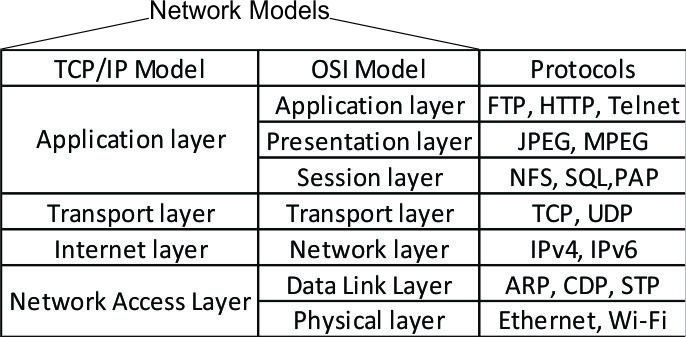
\includegraphics[height=4cm]{TVY-POS/ISO-OSI-TCP-IP/tcpip.jpg}
    \end{multicols}

    V koncových uzlech jsou implementovány všechny vrstvy pro kontrolu dat, v přechodových uzlech je implementována pouze síťová vrstva a vrstva síťového rozhraní.
    Komunikace probíhá mezi sousedními vrstvami nebo mezi stejnolehlými vrstvami.
    \begin{multicols}{2}
      Hlavička TCP protokolu: \\
      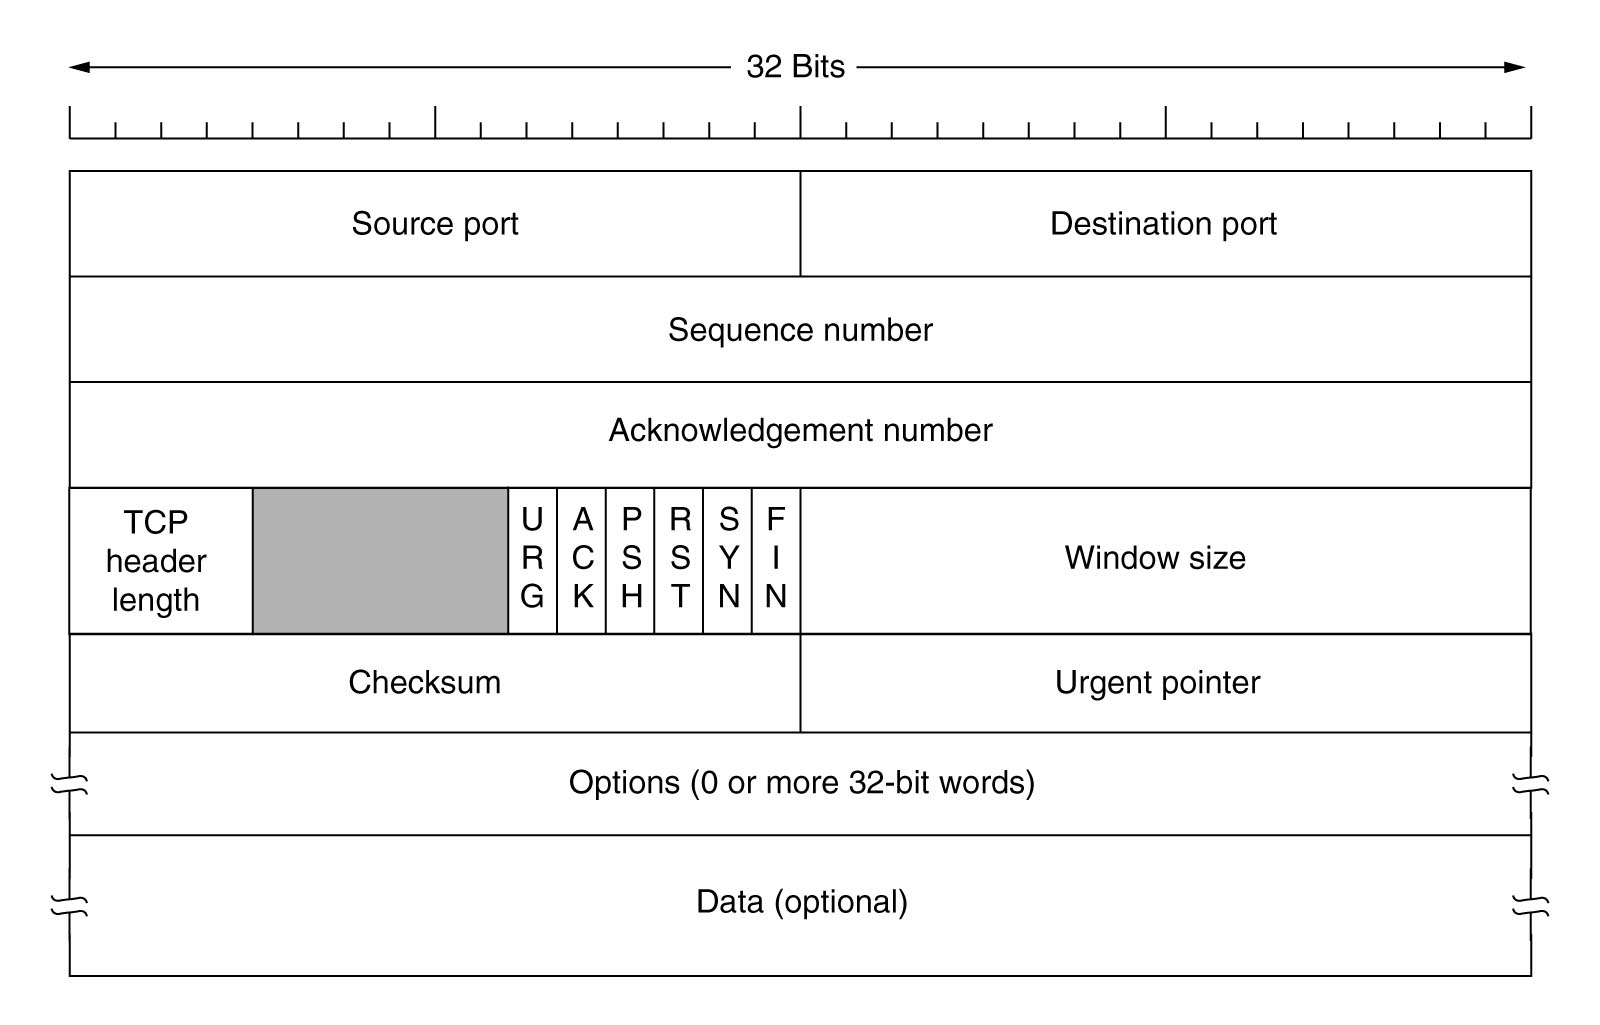
\includegraphics[width=\linewidth]{TVY-POS/ISO-OSI-TCP-IP/TCPheader.jpg}
      \columnbreak
      
      Pro navození komunikace
      \begin{enumerate}
        \item Klient vyšle na server požadavek na komunikaci s příznakem SYN, náhodným číslem sekvence (x) a číslem potvrzování 0.
        \item Server odešle klientovi datagram s číslem potvrzování x+1 a náhodným číslem sekvence (y), příznak zprávy nastaví na SYN, ACK.
        \item Klient odešle datagram s příznakem ACK, číslem sekvence x+1, číslem odpovědi y+1.
      \end{enumerate}
    \end{multicols}
    \begin{multicols}{2}
        Hlavička UDP protokolu: \\
        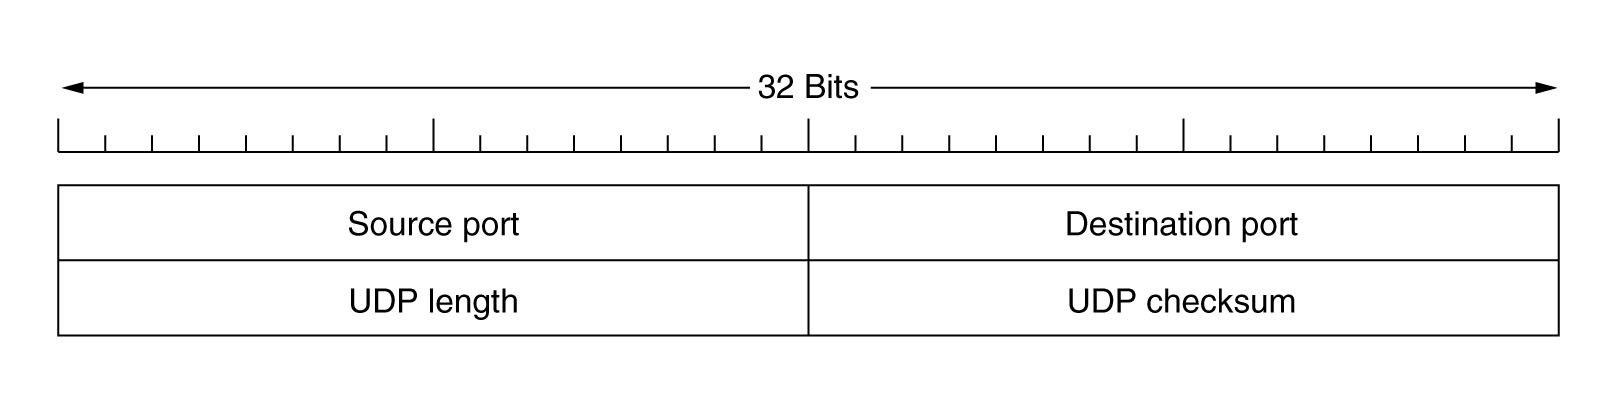
\includegraphics[width=\linewidth]{TVY-POS/ISO-OSI-TCP-IP/UDPheader.jpg}
        \columnbreak
        \newline
        Pro ukončení komunikace:
        \begin{enumerate}
          \item Klient odešle FIN
          \item Server odpoví ACK a pošle FIN
          \item Klient odpoví FIN = Konec
        \end{enumerate}
      \end{multicols}

  \subsection{IP}
    Univerzální přenosový protokol k nespolehlivému, nespojovanému přenosu dat mezi zdrojovým počítačem a příjemcem.
    Každé zařízení dostává nějakou indentifikaci v podobě IP adresy.
    Přenášená data se nazývají IP datagramy neboli IP pakety, každý paket obsahuje hlavičku, ve které nese metadata a vlastní přenášená data.
    Dnes se používají protokoly IPv4 a IPv6. \\
    Formát IP diagramu: \\
    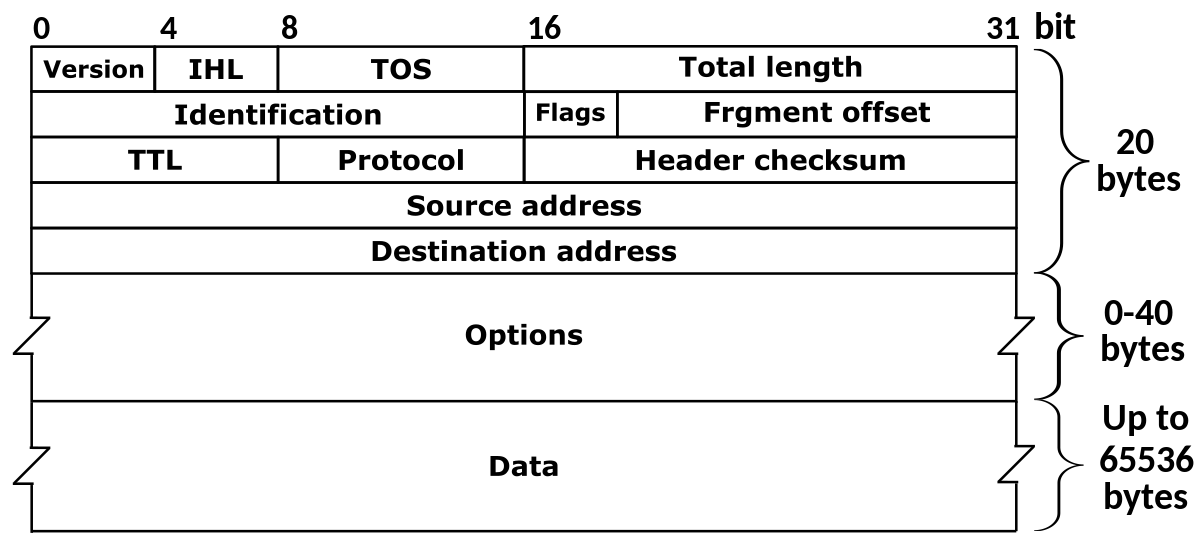
\includegraphics[height=5cm]{TVY-POS/ISO-OSI-TCP-IP/IPv4.png} \\
    Údaje hlavičky:
    \begin{tabbing}
      name ~~~~~~~~~~~~~~~~~~~~\= notes \kill
      \bfseries Údaje \>\bfseries Pozn.\\[2mm]
      Verze\>IPv4 nebo IPv6\\
      ToS,QoS\>Třída provozu, požadavky na přenos\\
      Identifikace\>Jednoznačné určení paketu při fragmentaci\\
      Příznaky\>Řízení fragmentace (more fragments, don't fragment)\\
      Offset\>Pozice fragmentu v původním paketu\\
      Time To Live\>Položka bránící zacyklení paketu, po průchodu směrovačem snížena\\
      \>jakmile = 0 je paket zahozen\\
      Protkol\>Číslo protokolu podle RFC\\
      Kontrolní součet\>Pokud nesouhlasí, je paket zahozen\\
      Volby\>Doplňující informace a požadavky (obvykle se nepoužívá)\\
    \end{tabbing}
    Pokud přenosová kapacita nestačí pro přenášená data, může IP některé pakety zahodit.
    Cesta není předem vytyčena a optimální cestu nachází každý uzel, přes který daný paket jde.
    Zpráva rozdělená na několik paketů nemusí dorazit ve stejném pořadí, jako byla poslána.
    Každý poškozený paket síťová vrstva zahodí.
    Požaduje-li aplikace spolehlivý přenos dat, jsou k dispozici protokoly vyšších vrstev.
    Při přenosu velkých dat se mohou data fragmentovat.
    Fragmentují se na vysílající stanici a defragmentují na přijímací.